% document's head

\phantom{42}
\vspace{20mm}

\begin{center}
    \LARGE \textsc{Лабораторная работа} \\
    \vspace{3 mm}
    \large Измерение частоты темнового счёта и шум-фактора твердотельного фотоумножителя SiPM
\end{center}

% \hrule

\phantom{42}

\begin{flushright}
    \begin{tabular}{rr}
    % written by:
        % \textbf{Источник}: 
        % & \href{__ссылка__}{__название__} \\
        % & \\
        % \textbf{Лектор}: 
        % & _ФИО_ \\
        % & \\
        \textbf{Автор работы}: 
        & Хоружий Кирилл \\ 
        & Кузнецова Арина \\
        & Евгений Дедков \\
        & Александр Двуреченский \\
        & Яушев Михаил  \\ 
        & \\
    % date:
        \textbf{От}: &
        \textit{\today}\\
    \end{tabular}
\end{flushright}

\thispagestyle{empty}

\vspace{10mm}


\subsection*{Цель работы}
Измерение частоты темнового счёта и шум-фактора твердотельного фотоумножителя SiPM.

\subsection*{Оборудование}
Источник-измеритель Keithley 236 (smu), измерительный модуль\,(фильтр низких частот, фотодетектор, фильтр высоких частот, усилитель), длинная линия с волновым сопротивлением 50\,Ом, осциллограф Tektronix TDS7104, пинцет.

\begin{figure}[h]
    \centering
    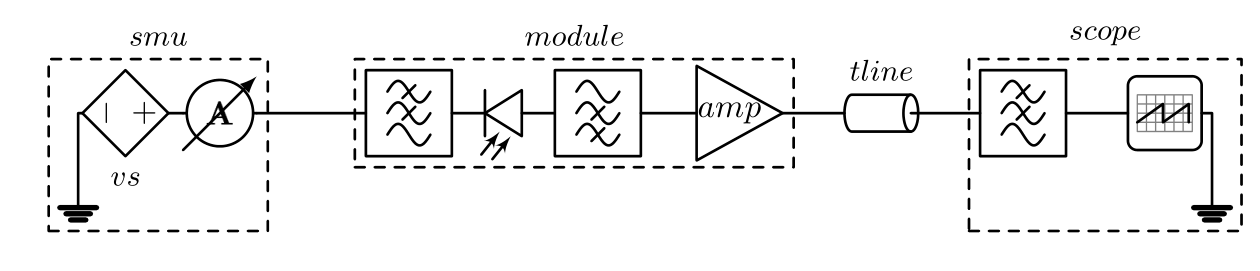
\includegraphics[width=0.5\textwidth]{figures/exp.png}
    \caption{Блок-схема измерительной установки}
    \label{fig:exp}
\end{figure}

Источник измеритель smu, состоящий из управляемого источника напряжения vs и измерителя тока, через фильтр низких частот измерительного модуля обеспечивает фотодетектор напряжением обратного смещения. 

Сигнал с фотодетектора проходит через фильтр высоких частот и усиливается при помощи amp. Сигнал с выход усилителя попадает в длинную линию и передается на вход осциллографа scope. 


\newpage
